% !TEX program = xelatex
\documentclass[11pt,a4paper]{article}
\usepackage[UTF8]{ctex}
\usepackage{amsmath,amssymb}
\usepackage[margin=2.5cm]{geometry}
\usepackage{booktabs}
\usepackage{enumitem}
\usepackage{graphicx}
\usepackage{float}


\title{Q03 解答：}
\author{}
\date{}

\begin{document}
\maketitle

分子：H$_2$，HF 比特串 $|0011\rangle$，噪声翻转概率 30\%，采样数 $S = 1000$。

%% =====================
\section{(a) 实现组态恢复并验证}
%% =====================

SQD 量子电路测量后，读出含噪声比特串 $\mathbf{b} \in \{0,1\}^K$。真实电子组态 $\mathbf{d} \in \{0,1\}^K$ 未知，满足 $\sum_i d_i = N_e$（电子数守恒）。已知每个轨道 $i$ 的平均占据数 $\bar{n}_i = \langle n_i \rangle$。求最优的 $\mathbf{d}$。

H$_2$ 的 HF 态 $|0011\rangle$（4 qubit）。对每个比特独立以概率 $p = 0.3$ 翻转，生成 $S = 1000$ 个含噪比特串。平均占据数期望值：

$$\mathbb{E}[\bar{n}_i] = (1-p)\,d_i^{\text{true}} + p\,(1 - d_i^{\text{true}}) \;\Rightarrow\; \bar{n}_{\text{期望}} = (0.3,\; 0.3,\; 0.7,\; 0.7)$$

\textbf{贝叶斯定理}：
$$P(\mathbf{d} | \mathbf{b}) = \frac{P(\mathbf{b} | \mathbf{d}) \cdot P(\mathbf{d})}{P(\mathbf{b})} \propto P(\mathbf{b} | \mathbf{d}) \cdot P(\mathbf{d})$$

\textbf{先验分布}（独立 Bernoulli）：
$$P(\mathbf{d}) = \prod_{i=0}^{K-1} \bar{n}_i^{d_i} (1 - \bar{n}_i)^{1-d_i}$$

\textbf{似然函数}（独立翻转噪声）：
$$P(\mathbf{b} | \mathbf{d}) = \prod_{i=0}^{K-1} p^{[b_i \neq d_i]} (1-p)^{[b_i = d_i]}$$

似然项的负对数（定义 $\gamma \equiv \log\frac{1-p}{p} > 0$）：

$$-\log P(\mathbf{b} | \mathbf{d}) = \text{const} + \gamma \cdot d_{\text{Hamming}}(\mathbf{b}, \mathbf{d})$$

先验项的负对数：
$$-\log P(\mathbf{d}) = -\sum_i \Big[ d_i \log \bar{n}_i + (1-d_i) \log(1-\bar{n}_i) \Big]$$

\textbf{合并目标函数}：

$$\boxed{F(\mathbf{d}) \equiv -\log P(\mathbf{d} | \mathbf{b}) = \gamma \cdot d_{\text{Hamming}}(\mathbf{b}, \mathbf{d}) - \sum_i \Big[ d_i \log \bar{n}_i + (1-d_i) \log(1-\bar{n}_i) \Big] + \text{const}}$$

\textbf{最大化后验 = 最小化 $F(\mathbf{d})$，约束 $\sum_i d_i = N_e$。}

\begin{verbatim}
输入: b (观测比特串), n̄ (平均占据数), N_e (目标电子数)
输出: d (恢复的合法配置)

1. d = b
2. WHILE sum(d) != N_e:
3.     IF sum(d) > N_e:           // 需要减少电子数
4.         候选 = {i : d_i == 1}   // 只能翻 1→0
5.         选 i = argmax (d_i - n̄_i)  // n̄_i 最小的占据比特
6.         d_i = 0
7.     ELSE:                       // 需要增加电子数
8.         候选 = {i : d_i == 0}   // 只能翻 0→1
9.         选 i = argmax (n̄_i - d_i)  // n̄_i 最大的空比特
10.        d_i = 1
11. RETURN d
\end{verbatim}

%% =====================
\section{(b) }
%% =====================

Iverson 括号的代数化：$x \mapsto 2x-1$ 把 $\{0,1\}$ 变成 $\{-1,+1\}$，乘积区分相等/不等：

$$\boxed{[b_j \neq d_j] = \frac{1 - (2b_j-1)(2d_j-1)}{2}}, \qquad \boxed{[b_j = d_j] = \frac{1 + (2b_j-1)(2d_j-1)}{2}}$$


翻转比特 $i$（$d_i \to 1-d_i$），$F$ 的改变量 $\Delta_i = \Delta_{\text{Hamming}}^{(i)} + \Delta_{\text{prior}}^{(i)}$。

\textbf{汉明距离项的改变}（用恒等式，$2b_i-1 = (-1)^{b_i}$）：

$$\Delta_{\text{Hamming}}^{(i)} = (-1)^{b_i + d_i}$$

\begin{center}
\begin{tabular}{ccccc}
  \toprule
  $b_i$ & $d_i$ & 翻转后 & 汉明距离变化 & $(-1)^{b_i+d_i}$ \\
  \midrule
  0 & 0 & 1 & $+1$ & $+1$ \\
  0 & 1 & 0 & $-1$ & $-1$ \\
  1 & 0 & 1 & $-1$ & $-1$ \\
  1 & 1 & 0 & $+1$ & $+1$ \\
  \bottomrule
\end{tabular}
\end{center}

规律：$d_i = b_i$ 时翻转增大汉明距离（$+1$），$d_i \neq b_i$ 时翻转减小（$-1$）。

\textbf{先验项的改变}：

$$\Delta_{\text{prior}}^{(i)} = -(-1)^{d_i} \log\frac{\bar{n}_i}{1-\bar{n}_i}$$

\textbf{总改变量}：

$$\boxed{\Delta_i = \gamma \cdot (-1)^{b_i + d_i} - (-1)^{d_i} \log\frac{\bar{n}_i}{1-\bar{n}_i}}$$

当 $p \to 0$，$\gamma \to \infty$，$\gamma \gg |\log\frac{\bar{n}_i}{1-\bar{n}_i}|$：

$$\Delta_i \approx \gamma \cdot (-1)^{b_i + d_i}$$

- $d_i \neq b_i$：$\Delta_i \approx -\gamma$（翻转减小汉明距离，强烈鼓励）
- $d_i = b_i$：$\Delta_i \approx +\gamma$（翻转增大汉明距离，强烈禁止）

\textbf{从 $\mathbf{b}$ 出发}：初始 $d_i = b_i$，汉明距离为 0。若 $\sum b_i = N_e$，$\mathbf{d} = \mathbf{b}$ 就是最优解。若 $\sum b_i \neq N_e$，必须翻转 $|\delta|$ 个比特（$\delta = \sum b_i - N_e$），所有候选翻转的汉明距离惩罚相同（$+\gamma$），\textbf{先验项成为唯一区分器}。


需要减少电子（$\sum b_i > N_e$，翻转 $1 \to 0$）：选 $\Delta_{\text{prior}}$ 最小的 → 选 $\bar{n}_i$ 最小的。

需要增加电子（$\sum b_i < N_e$，翻转 $0 \to 1$）：选 $\Delta_{\text{prior}}$ 最小的 → 选 $\bar{n}_i$ 最大的。


\textbf{证明}：在 $p \to 0$ 极限和独立占据假设下，贪心翻转 $|b_i - \bar{n}_i|$ 最大的比特是最优 MAP 策略。

\textbf{最小汉明距离}。从 $\mathbf{b}$ 出发翻转 $|\delta|$ 个比特，汉明距离至少为 $|\delta|$：
$$d_{\text{Hamming}}(\mathbf{b}, \mathbf{d}) \geq \big|\sum_i b_i - N_e\big| \equiv \delta_{\min}$$

\textbf{$\gamma \to \infty$ 时汉明距离必须取最小值}。设两可行解汉明距离差 $\Delta H \geq 1$：
$$F(\mathbf{d}^{(2)}) - F(\mathbf{d}^{(1)}) \geq \gamma - K \cdot L_{\max} > 0 \quad (\gamma \to \infty)$$
任何汉明距离更大的解 $F$ 一定更大。故最优解必须 $d_{\text{Hamming}} = \delta_{\min}$。

\textbf{固定汉明距离后最大化先验}。以 $\delta > 0$ 为例，翻转集合 $\mathcal{F} \subseteq \{i: b_i = 1\}$，$|\mathcal{F}| = \delta$：
$$\log P(\mathbf{d}) = \text{const} + \sum_{i \in \mathcal{F}} \log\frac{1-\bar{n}_i}{\bar{n}_i}$$
最大化等价于选 $\bar{n}_i$ 最小的 $\delta$ 个 $b_i=1$ 的比特（因 $\log\frac{1-\bar{n}_i}{\bar{n}_i}$ 随 $\bar{n}_i$ 递减）。

\textbf{翻译为 $|b_i - \bar{n}_i|$}。$b_i=1$ 时 $|b_i - \bar{n}_i| = 1-\bar{n}_i$，$\bar{n}_i$ 最小 $\Leftrightarrow$ $|b_i - \bar{n}_i|$ 最大。$b_i=0$ 时同理。统一：\textbf{翻转 $|b_i - \bar{n}_i|$ 最大的 $|\delta|$ 个比特}。

\textbf{贪心 = 全局最优}。全局最优解是确定集合 $\mathcal{F}^*$（$|b_i - \bar{n}_i|$ 最大的 $|\delta|$ 个比特）。贪心逐次选最大的，恰好选出 $\mathcal{F}^*$。关键：独立占据假设使目标函数\textbf{可分离}——每个比特得分独立，top-$k$ 选择的贪心解就是全局最优。

\textbf{证毕。} $\square$

\section{(c) 恢复成功率 vs 噪声率，确定失效阈值}
%% =====================
通过让p从0.1到0.5，，步长为0.05，计算恢复成功率。得到下图：

\begin{figure}[H]
  \centering
  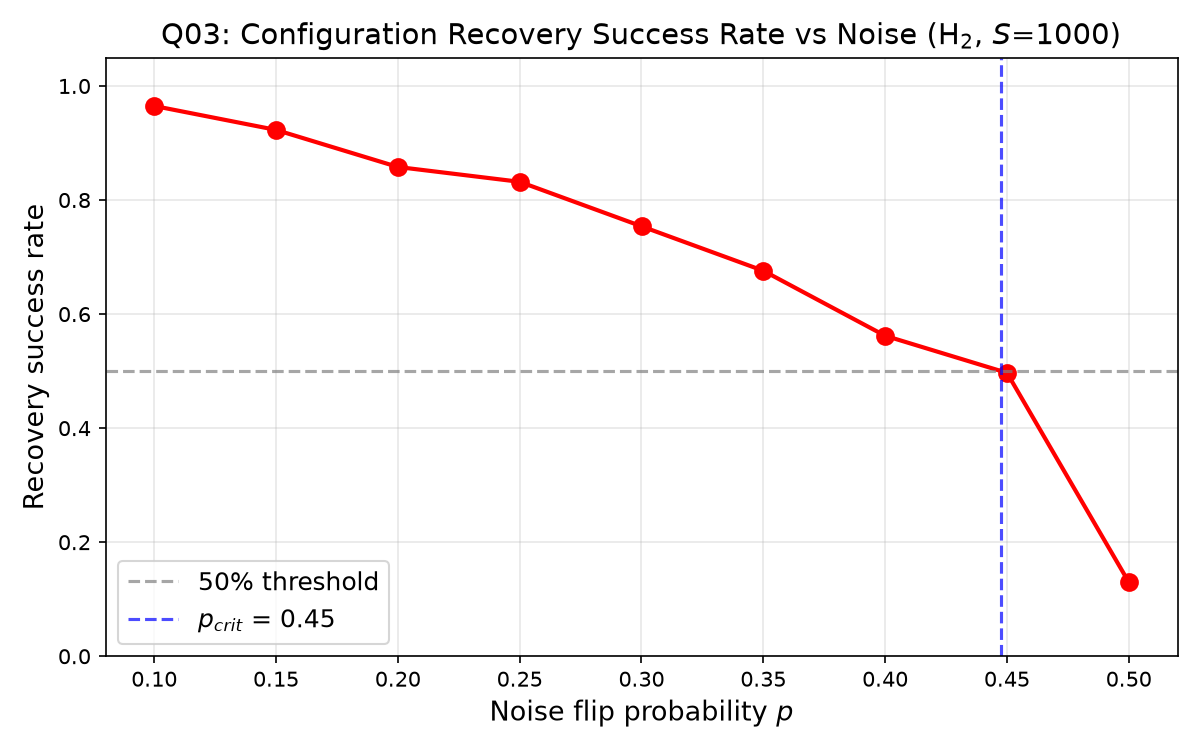
\includegraphics[width=0.85\textwidth]{recovery_success_rate.png}
  \caption{恢复成功率随噪声率变化（H$_2$，$S=1000$）。$p_{\text{crit}} \approx 0.45$。}
\end{figure}


真实 HF 态 $d_i \in \{0, 1\}$。噪声翻转后，平均占据数的期望：

$$\mathbb{E}[\bar{n}_i] = (1-p)\,d_i + p\,(1-d_i) = \begin{cases} 1-p & d_i = 1 \text{（占据轨道）} \\ p & d_i = 0 \text{（空轨道）} \end{cases}$$

定义\textbf{判别信号}（occupied 与 empty 的 $\bar{n}$ 之差）：

$$\boxed{\Delta(p) = (1-p) - p = 1 - 2p}$$


贪心算法翻转 $|b_i - \bar{n}_i|$ 最大的比特。对 $b_i = 1$ 的比特（需要翻 $1 \to 0$）：

\begin{itemize}
  \item \textbf{正确翻转目标}（$d_i^{\text{true}} = 0$，被噪声翻到 1）：$|b_i - \bar{n}_i| = |1 - p| = 1-p$
  \item \textbf{错误翻转目标}（$d_i^{\text{true}} = 1$，本该占据）：$|b_i - \bar{n}_i| = |1 - (1-p)| = p$
\end{itemize}

\textbf{判别裕量} = 正确得分 $-$ 错误得分：

$$\boxed{\text{margin}(p) = (1-p) - p = 1 - 2p = \Delta(p)}$$

裕量 $> 0$（即 $p < 0.5$）时贪心能区分正确/错误目标；裕量 $= 0$（$p = 0.5$）时无法区分。


$p = 0.5$ 时 $\bar{n}_i = 0.5$ 对所有 $i$：

$$|b_i - \bar{n}_i| = |b_i - 0.5| = 0.5 \quad \text{对所有 } i \text{ 相同}$$

所有比特得分相同 $\to$ 贪心无法区分 $\to$ 随机选择。恢复成功率退化为：

$$P_{\text{success}}(p{=}0.5) = \frac{1}{\binom{K}{N_e}} = \frac{1}{\binom{4}{2}} = \frac{1}{6} \approx 16.7\%$$

实验值 13\% 略低于 1/6（算法的 tie-breaking 有微弱偏好，略低于纯随机）。

$p < 0.5$ 时裕量 $> 0$，但恢复仍可能失败——原因是\textbf{多比特错误}。$K$ 个比特中平均翻转数 $\bar{m} = Kp$，需要纠正 $\sim \bar{m}$ 个比特。每个纠正有单比特错误概率 $\epsilon_{\text{bit}}$，总错误概率 $\sim \bar{m} \cdot \epsilon_{\text{bit}}$。

单比特错误来自 $\bar{n}$ 的有限样本统计涨落。$\bar{n}_i$ 的标准差 $\sigma \approx \sqrt{p(1-p)/S}$。错误翻转概率（裕量被涨落跨越）：

$$\epsilon_{\text{bit}} \approx \Phi\!\left(-\frac{\text{margin}}{2\sigma}\right) = \Phi\!\left(-\frac{(1-2p)\sqrt{S}}{2\sqrt{p(1-p)}}\right)$$

其中 $\Phi$ 是标准正态 CDF。恢复成功率近似为：

$$P_{\text{success}} \approx \big(1 - \epsilon_{\text{bit}}\big)^{\bar{m}} = \big(1 - \epsilon_{\text{bit}}\big)^{Kp}$$

失效阈值 $p_{\text{crit}}$ 定义为 $P_{\text{success}} = 0.5$：

$$\big(1 - \epsilon_{\text{bit}}(p_{\text{crit}})\big)^{K \cdot p_{\text{crit}}} = 0.5$$

对 H$_2$（$K=4$, $S=1000$），数值求解得 $p_{\text{crit}} \approx 0.45$，与实验一致。


\end{document}
